\let\negmedspace\undefined
\let\negthickspace\undefined
\documentclass[journal]{IEEEtran}
\usepackage[a4paper, margin=10mm, onecolumn]{geometry}
\usepackage{lmodern} % Ensure lmodern is loaded for pdflatex
\usepackage{tfrupee} % Include tfrupee package

\setlength{\headheight}{1cm} % Set the height of the header box
\setlength{\headsep}{0mm}  % Set the distance between the header box and the top of the text

\usepackage{gvv-book}
\usepackage{gvv}
\usepackage{cite}
\usepackage{amsmath,amssymb,amsfonts,amsthm}
\usepackage{algorithmic}
\usepackage{graphicx}
\usepackage{float}
\usepackage{textcomp}
\usepackage{xcolor}
\usepackage{txfonts}
\usepackage{listings}
\usepackage{enumitem}
\usepackage{mathtools}
\usepackage{gensymb}
\usepackage{comment}
\usepackage[breaklinks=true]{hyperref}
\usepackage{tkz-euclide} 
\usepackage{listings}
% \usepackage{gvv}                                        
\def\inputGnumericTable{}                                 
\usepackage[latin1]{inputenc}                                
\usepackage{color}                                            
\usepackage{array}                                            
\usepackage{longtable}                                       
\usepackage{calc}                                             
\usepackage{multirow}                                         
\usepackage{hhline}                                           
\usepackage{ifthen}                                           
\usepackage{lscape}
\usepackage{tikz}
\usetikzlibrary{patterns}

\begin{document}

\bibliographystyle{IEEEtran}
\vspace{3cm}

\title{4.12.1}
\author{EE25BTECH11064 - Yojit Manral}

\maketitle
% \maketitle
% \newpage
% \bigskip
{\let\newpage\relax\maketitle}
\renewcommand{\thefigure}{\theenumi}
\renewcommand{\thetable}{\theenumi}
\setlength{\intextsep}{10pt} % Space between text and float

\textbf{Question:}\\
For which values of a and b does the following pair of linear equations have an
infinite number of solutions?
\begin{align*}
    2x + 3y &= 7 \\
    (a - b)x + (a + b)y &= 3a + b - 2
\end{align*}

\textbf{Solution:}\\
$\rightarrow$ The equation of the lines can be written as
\begin{align}
    \vec{n_1}^{T}\vec{x} &= c_1 \\
    \vec{n_2}^{T}\vec{x} &= c_2
\end{align}
\hspace{0.3cm} where,
\begin{align}
    \vec{n_1} &= \myvec{2\\3} \\
    \vec{n_2} &= \myvec{a-b\\a+b} \\
    c_1 &= 7 \\
    c_2 &= 3a + b -2
\end{align}
$\rightarrow$ For two lines to have infinite solutions,,
\begin{align}
    \vec{n_1} &= \alpha \vec{n_2} \\
    c_1 &= \alpha c_2 \\
    \implies c_2 \vec{n_1} &= c_1 \vec{n_2}
\end{align}
$\rightarrow$ Substituting the values from (3), (4), (5), and (6) in (9)
\begin{align}
    (3a + b - 2)\myvec{2\\3} &= 7 \myvec{a-b\\a+b} \\
    \myvec{6a + 2b\\9a + 3b} - \myvec{7a-7b\\7a+7b} = \myvec{-a + 9b\\2a - 4b} &= \myvec{4\\6} \\
    \implies \myvec{-1&&9\\2&&-4}\myvec{a\\b} &= \myvec{4\\6}
\end{align}
$\rightarrow$ Using row transformations
\begin{align}
    \myvec{-1&&9\\2&&-4}\myvec{a\\b} = \myvec{4\\6} &\xrightarrow{R_1 \leftrightarrow -R_1} \myvec{1&&-9\\2&&-4}\myvec{a\\b} = \myvec{-4\\6} \\
    &\xrightarrow{R_2 \leftrightarrow R_2 - 2R_1} \myvec{1&&-9\\0&&14}\myvec{a\\b} = \myvec{-4\\14} \\
    &\xrightarrow{R_2 \leftrightarrow (1/14)R_2} \myvec{1&&-9\\0&&1}\myvec{a\\b} = \myvec{-4\\1} \\
    &\xrightarrow{R_1 \leftrightarrow R_1 + 9R_2} \myvec{1&&0\\0&&1}\myvec{a\\b} = \myvec{5\\1} \\
    \implies &\myvec{a\\b} = \myvec{5\\1} \implies a = 5 \text{ and } b = 1
\end{align}
\begin{figure}[h!]
   \centering
   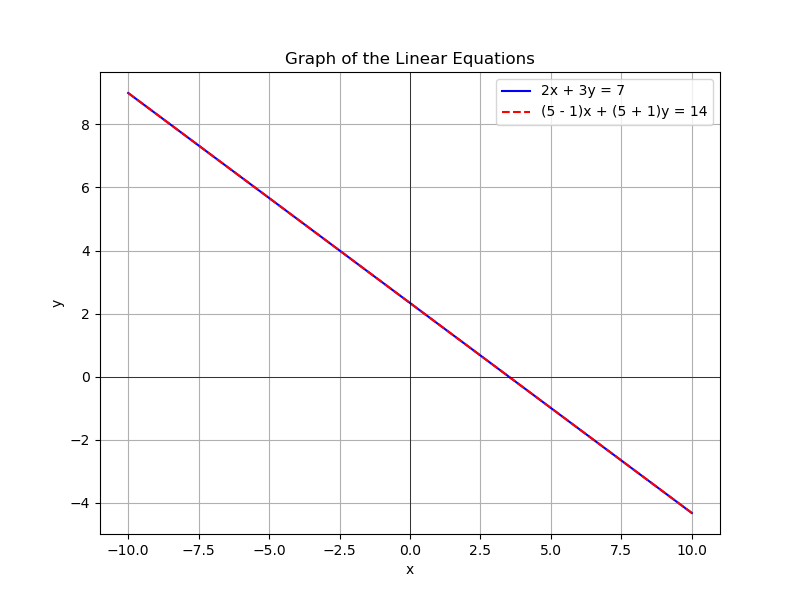
\includegraphics[width=0.8\linewidth]{figs/01.png}
   \caption{Plot of the given lines}
   \label{Plot_1}
\end{figure}
\end{document}
